\documentclass[conference]{IEEEtran}
\IEEEoverridecommandlockouts
% The preceding line is only needed to identify funding in the first footnote. If that is unneeded, please comment it out.
\usepackage{cite}
\usepackage{amsmath,amssymb,amsfonts}
\usepackage{algorithmic}
\usepackage{graphicx}
\usepackage{textcomp}
\usepackage{xcolor}
\usepackage{hyperref}
\usepackage{subfig}
%\DeclareUnicodeCharacter{200B}{I~AM~HERE!!!!}

\def\BibTeX{{\rm B\kern-.05em{\sc i\kern-.025em b}\kern-.08em
    T\kern-.1667em\lower.7ex\hbox{E}\kern-.125emX}}
\begin{document}

\title{Sistemi e Architetture per Big Data - AA 2020/2021 \\
	\LARGE \emph{Secondo progetto}}

\author{\IEEEauthorblockN{Giuseppe Lasco}
\IEEEauthorblockA{\textit{Dipartimento di Ingegneria dell'Informazione} \\
\textit{Universit\`{a} degli studi di Roma "Tor Vergata"
}\\
Roma, Italia \\
giuseppe.lasco17@gmail.com}
\and
\IEEEauthorblockN{Marco Marcucci}
\IEEEauthorblockA{\textit{Dipartimento di Ingegneria dell'Informazione} \\
\textit{Universit\`{a} degli studi di Roma "Tor Vergata"
}\\
Roma, Italia \\
marco.marcucci96@gmail.com}

}

\maketitle

\begin{abstract}
Questo documento riporta i dettagli implementativi
riguardanti l'analisi mediante \emph{Flink} del dataset relativo a dati provenienti da
dispositivi Automatic Identification System (AIS) contenenti informazioni riguardo lo stato di navi in movimento per garantire la sicurezza di quest'ultime in mare e nei porti. Viene, inoltre, descritta l'architettura
a supporto dell'analisi e gli ulteriori \emph{framework} utilizzati.
\end{abstract}

\section{\textbf{Introduzione}}
L'analisi effettuata si pone lo scopo di rispondere a delle
query relative a classifiche e statistiche riguardanti le navi e le tratte presenti nel dataset.\\

\subsection*{\textbf{Dataset}} 
Il dataset preso in considerazione \`{e} \textit{prj2\_dataset.csv}, il quale contiene dati rigurdanti gli identificativi e le caratteristiche istantanee delle navi e delle tratte. I campi di interesse sono:
\begin{itemize}
\item \textbf{ID}: stringa esadecimale che rappresenta l’identificativo della nave;
\item \textbf{SHIP TYPE}: numero intero che rappresenta la tipologia della nave
\item \textbf{LON}: numero in virgola mobile che rappresenta la coordinata cartesiana in gradi decimali della
longitudine data dal GPS;
\item \textbf{LAT}: numero in virgola mobile che rappresenta la coordinata cartesiana in gradi decimali della latitudine data dal sistema GPS;
\item \textbf{TIMESTAMP}: rappresenta l’istante temporale della segnalazione dell’evento AIS; il timestamp è
espresso con il formato GG-MM-YY hh:mm:ss (giorno, mese, anno, ore, minuti e secondi dell’evento);
\item \textbf{TRIP ID}: stringa alfanumerica che rappresenta l’identificativo del viaggio; è composta dai primi 7
caratteri (inclusi 0x) di SHIP ID, concatenati con la data di partenza e di arrivo.
\end{itemize}
\par La
frequenza di produzione di tali dati è in funzione dello stato di moto, con un periodo temporale variabile tra i 2 secondi in fase di manovra a 5 minuti in fase di navigazione ad alta velocità. Inoltre, l'area marittima è limitata alla zona del Mar Mediterraneo descritta dalle seguente coordinate: LON $\in$ [-6.0, 37.0] LAT $\in$ [32.0, 45.0].
Tale area è stata suddivisa in celle rettangolari di uguale dimensione; i settori di LAT vengono identificati dalle lettere che vanno da A a J, mentre i settori di LON dai numeri interi che vanno da 1 a 40. Ad ogni cella è associato un \emph{id} dato dalla combinazione della lettera del
settore LAT e dal numero di settore LON.
\subsection*{\textbf{Query}}
L'obiettivo di questo progetto \`{e} quello di implementare ed eseguire tre query utilizzando \emph{Flink}.

\par La prima query ha come scopo quello di calcolare, per il Mar Mediterraneo Occidentale, il numero medio giornaliero  di navi militari, navi per trasporto passeggeri, navi cargo e le restanti tipologie, utilizzando finestre temporali di tipo \emph{Tumbling} da 7 giorni e da 1 mese.

\par La seconda query consiste nel determinare le prime 3 celle per le quali il grado di frequentazione \`{e} pi\`{u} alto, nelle due fascie orarie 00:00-11:59 e 12:00-23:59, Mar Mediterraneo Occidentale ed Orientale. il grado di frequentazione di una cella viene calcolato come il numero di navi diverse che attraversano la cella nella fascia oraria in esame. Sono state utilizzate finestre temporali a 7 giorni e 1 mese.

\par L'ultima query consiste nel determinare le prime 5 tratte per cui la distanza percorsa fino a quel momento \`{e} pi\`{u} alta. Per il calcolo della distanza è stata considerata la distanza euclidea.

\subsection*{\textbf{Framework}}
Come \emph{framework} di processamento stream \`{e} stato utilizzato \emph{Apache Flink} che riceve i dati dal sistema di messaging \emph{Apache Kafka}. 

\section{\textbf{Architettura}}
L'architettura si compone di due container \emph{Docker}, su cui eseguono i servizi di \emph{Apache Zookeeper} e \emph{Apache Kafka} che comunicano tra di loro attraverso la stessa rete, creata appositamente dal servizio \emph{Docker Compose}. Inoltre, sempre sulla stessa macchina, una JVM ospita l'esecuzione di \emph{Apache Flink} e un processo \emph{Java} immette i dati nel sistema di Publish/Subscribe.

\begin{figure}[htbp]
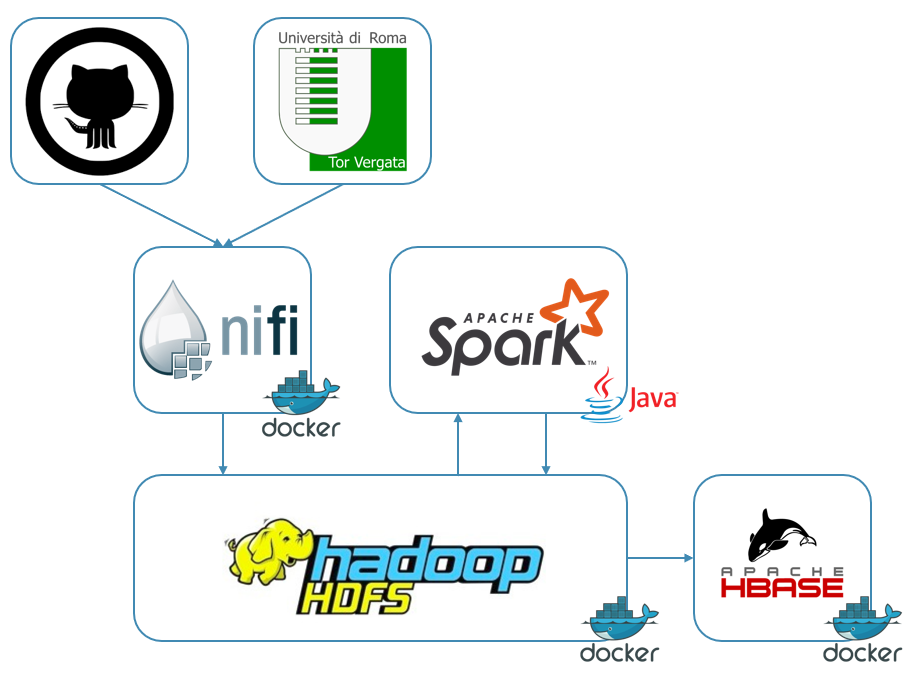
\includegraphics[scale=0.36]{Screenshot/arch.png}
\caption{Schema dell'architettura}\label{figura:architettura}
\label{fig}
\end{figure}

\subsection*{\textbf{Producer}}
Il Producer si occupa di leggere il ​dataset, mantenuto in un
file CSV locale, e di pubblicarne il contenuto presso il
topiche di Kafka (query) da cui \emph{Flink} recupera i dati. La scrittura sulla
topica viene effettuata riga per riga a intervalli variabili, proporzionali ai timestamp reali presenti nel dataset, al fine di simulare una
vera sorgente di dati ​real time ​accelerata. L'ordinamento del dataset \`{e} stato effettuato utilizzando una struttura dati che permette di ordinare all'inserimento dei record, ovvero la \emph{TreeMap}. La gestione di chiavi uguali (timestamp) \`{e} stata effettuata utilizzando come valore della coppia key-value della \emph{TreeMap}, una lista, popolata dai record da inviare, in modo da non perdere occorrenze.
Per garantire la corretta esecuzione del processamento su
\emph{Flink} in base all'​ event time,​ \`{e} stato necessario
estrarre la data di occorrenza dell'evento di ogni riga e
impostarla come ​timestamp della relativa tupla alla
pubblicazione sulla topica. 

\subsection*{\textbf{Apache Kafka}}
\emph{Kafka} è il sistema di messaggistica di tipo ​publish-subscribe
utilizzato per l'ingestion di dati nei sistemi di processamento
e per l'export dei risultati. Il ​cluster, realizzato con \emph{Docker
Compose}, prevede un​ container con \emph{Zookeeper}, necessario
per la coordinazione, e altri tre​ container con la funzione di
\emph{Kafka broker}. Sono state create 7 \emph{topiche}: una per le tuple
in input a Flink, due per l'output della prima query (settimanale e
mensile), due per l'output della seconda ​query (settimanale e mensile) e altrettante per quello della terza query (per un'ora e per due ore). Per incrementare la tolleranza ai guasti, ogni \emph{Kafka ​topic} è impostata per avere un grado di replicazione pari a 2 (una replica \emph{​leader} ed una replica
\emph{follower}) e, allo stesso tempo, una sola partizione. La scelta
della singola partizione è dovuta alla necessità di
mantenere le tuple ordinate all’interno del sistema di
messaggistica; in \emph{Kafka}, infatti, la garanzie di ordinamento
sono valide soltanto nell’ambito di una singola partizione.


\subsection*{\textbf{Apache Flink}}
\emph{Flink} \`{e} il framework di \emph{data stream processing} utilizzato per
l'esecuzione delle tre query precedentemente descritte.
I dati necessari al processamento sono presi direttamente
dalla \emph{topica} query in \emph{Kafka}. L'\emph{event time} viene determinato in automatico da \emph{Flink} recuperandolo dal campo \emph{timestamp} del record \emph{Kafka}. Il flusso cos\`{i} ottenuto rappresenta lo ​ stream che le ​ query
devono manipolare al fine di calcolare le statistiche
richieste.
Al fine di preprocessare i dati ed eseguire le \emph{query}, viene utilizzato \emph{Apache Flink} in locale, tramite lo script \texttt{\$FLINK\_HOME/bin/flink run}.
Di seguito viene mostrata la topologia che sarà
successivamente descritta più nel dettaglio.

\begin{figure}[htbp]
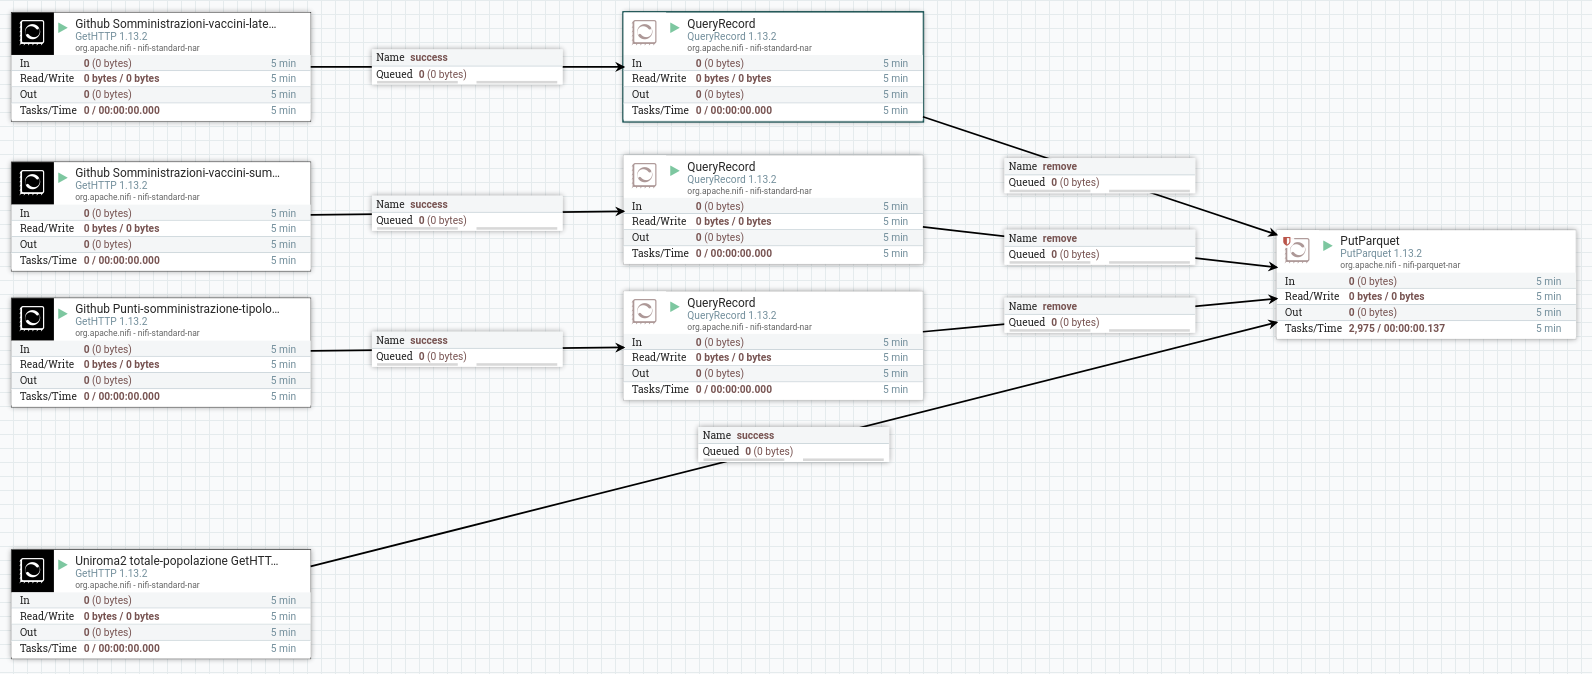
\includegraphics[scale=0.16]{Screenshot/Nifi.png}
\caption{NiFi template}\label{figura:template}
\label{fig}
\end{figure}


\section{\textbf{Query}}
\par Al fine di effettuare le query \`{e} stato necessario uno step di preprocessamento. Lo stream in ingresso viene generato utilizzando un consumer che riceve i dati dalla topica \emph{query}. I \emph{record} vengono trasformati in oggetti di tipo \emph{ShipData} contenenti le informazioni necessarie al processamento delle richieste; in particolare viene definita la cella e la sezione del Mar Mediterraneo (Occidentale o Orientale) di appartenenza a partire dalle coordinate. Una operazione di filtraggio assicura che i dati rientrino nella porzione di mare indicata dalla traccia. Lo stream di oggetti \emph{ShipData} in uscita viene, in seguito, dato in ingresso alle topologie di processamento delle query.
\subsection*{\textbf{Query 1}}
Per quanto riguarda la prima query, il processamento inizia filtrando i record, in modo da prenderer in considerazione solo quelli relativi al Mar Mediterraneo Occidentale.
Il processamento tramite \emph{Flink} prosegue sfruttando le
finestre temporali di tipo \emph{tumbling}
settimanali e mensili, parallelizzando attraverso il \emph{keyBy} per cella. Su tutte le finestre viene applicata una funzione di \emph{aggregate} personalizzata che permette, al contrario della \emph{process},​ di aggiornare le statistiche della \emph{​window} ogni volta
che una tupla le viene assegnata; questa accortezza
consente di evitare picchi di carico dovuti alla computazione in blocco di tutte le tuple assegnate a una finestra al completamento della stessa. In particolare, la funzione di aggregate permette di contare il numero di navi di un certo tipo passanti per una determinata cella nel periodo della finestra. Infine, attraverso una \emph{ProcessWindowFunction} user defined, si \`{e} prelevato il timestamp relativo all'inizio della finestra. Una \emph{map} ha permesso di formattare correttamente i dati da passare al \emph{sink}.


\subsection*{\textbf{Query 2}}
Per quanto riguarda la seconda query, il processamento tramite \emph{Flink} inizia sfruttando le
finestre temporali di tipo \emph{tumbling}
settimanali e mensili, parallelizzando attraverso il \emph{keyBy} per cella. Su tutte le finestre viene applicata una funzione di \emph{aggregate} personalizzata che permette di contare il numero di navi distinte passanti per una determinata cella nel periodo della finestra considerando le fasce orarie 00:00-11:59, 12:00-23:59 e Mar Mediterraneo Occidentale ed Orientale. Infine, attraverso una \emph{ProcessWindowFunction} user defined, si \`{e} prelevato il timestamp relativo all'inizio della finestra. Una finestra di tipo \emph{WindowAll} \`{e} stata necessaria al fine di generare la classifica delle celle pi\`{u} frequentate relative ad una certa zona di mare e una determinata fascia oraria. Una \emph{map} ha permesso di formattare correttamente i dati da passare al \emph{sink}.


\subsection*{\textbf{Query 3}}
Per quanto riguarda l'ultima query, il processamento tramite \emph{Flink} inizia sfruttando le
finestre temporali di tipo \emph{tumbling}
di una e due ore, parallelizzando attraverso il \emph{keyBy} per tripId. Su tutte le finestre viene applicata una funzione di \emph{aggregate} personalizzata che permette calcolare la distanza percorsa dalla nave in questione, tenendo traccia delle coordinate relative al record precedende, in modo da poter calcolare la distanza euclidea tra i punti e sommarla alla distanza cumulata fino a quel momento. Infine, attraverso una \emph{ProcessWindowFunction} user defined, si \`{e} prelevato il timestamp relativo all'inizio della finestra. Una finestra di tipo \emph{WindowAll} \`{e} stata necessaria al fine di generare la classifica dei viaggi con distanza coperta maggiore nel tempo della finestra. Una \emph{map} ha permesso di formattare correttamente i dati da passare al \emph{sink}.

\section{\textbf{Benchmark}}
L'esecuzione del progetto e la valutazione delle prestazioni sono state eseguite su \emph{Linux Mint 20.1 Cinnammon}, \emph{CPU AMD Ryzen 5 3600}, 6 core, 12 thread e 16 GB di RAM, con archiviazione su \emph{SSD}. \\
\begin{table}[htbp]
\caption{Latenze e throughput}
\begin{center}
    \begin{tabular}{|c|c|c|}
    \hline
    \textbf{Query} & \textbf{Throughput (tuple/sec)} & \textbf{Latenza (sec/tupla)}  \\ \hline
    Query 1 weekly & 330.751 & 0.003  \\ \hline
    Query 1 monthly & 381.912 & 0.003  \\ \hline
    Query 2 weekly & 320.114 & 0.003  \\ \hline
    Query 2 monthly & 344.525 & 0.003  \\ \hline
    Query 3 one hour & 330.472 & 0.003  \\ \hline
    Query 3 two hour & 344.525 & 0.003  \\ \hline
    \multicolumn{3}{l}{$^{\mathrm{*}}$Le metriche si riferiscono alla durata complessiva del replay di 10 secondi}
    \end{tabular}
\label{tab1}
\end{center}
\end{table}
\par Per poter eseguire una valutazione sperimentale dei
benchmark di ogni operatore, \`{e} stata utilizzata, per ognuno
di essi, una struttura tenente conto sia del numero di tuple
processate che del tempo impiegato; l'accesso a tale
struttura \`{e} effettuato, per evitare inconsistenze nel caso di
aggiornamenti simultanei da parte di operatori replicati,
mediante l’utilizzo di metodi \texttt{​synchronized​}.
In tabella~\ref{tab1} sono riportati i throughput e le latenze medie di processamento dei singoli eventi che attraversano la topologia per le tre query. 

\begin{thebibliography}{00}
\bibitem{b1} \url{https://spark.apache.org/docs/latest/}
\bibitem{b2} \url{https://stackoverflow.com/}
\bibitem{b3} \url{https://nifi.apache.org/}
\bibitem{b4} \url{https://hadoop.apache.org/docs/stable/}
\bibitem{b5} \url{http://spark.apache.org/docs/latest/ml-guide.html}
\bibitem{b6} \url{https://commons.apache.org/proper/commons-math/javadocs/api-3.3/org/apache/commons/math3/stat/regression/SimpleRegression.html}
\end{thebibliography}

\end{document}
